\documentclass[1p]{elsarticle_modified}
%\bibliographystyle{elsarticle-num}

%\usepackage[colorlinks]{hyperref}
%\usepackage{abbrmath_seonhwa} %\Abb, \Ascr, \Acal ,\Abf, \Afrak
\usepackage{amsfonts}
\usepackage{amssymb}
\usepackage{amsmath}
\usepackage{amsthm}
\usepackage{scalefnt}
\usepackage{amsbsy}
\usepackage{kotex}
\usepackage{caption}
\usepackage{subfig}
\usepackage{color}
\usepackage{graphicx}
\usepackage{xcolor} %% white, black, red, green, blue, cyan, magenta, yellow
\usepackage{float}
\usepackage{setspace}
\usepackage{hyperref}

\usepackage{tikz}
\usetikzlibrary{arrows}

\usepackage{multirow}
\usepackage{array} % fixed length table
\usepackage{hhline}

%%%%%%%%%%%%%%%%%%%%%
\makeatletter
\renewcommand*\env@matrix[1][\arraystretch]{%
	\edef\arraystretch{#1}%
	\hskip -\arraycolsep
	\let\@ifnextchar\new@ifnextchar
	\array{*\c@MaxMatrixCols c}}
\makeatother %https://tex.stackexchange.com/questions/14071/how-can-i-increase-the-line-spacing-in-a-matrix
%%%%%%%%%%%%%%%

\usepackage[normalem]{ulem}

\newcommand{\msout}[1]{\ifmmode\text{\sout{\ensuremath{#1}}}\else\sout{#1}\fi}
%SOURCE: \msout is \stkout macro in https://tex.stackexchange.com/questions/20609/strikeout-in-math-mode

\newcommand{\cancel}[1]{
	\ifmmode
	{\color{red}\msout{#1}}
	\else
	{\color{red}\sout{#1}}
	\fi
}

\newcommand{\add}[1]{
	{\color{blue}\uwave{#1}}
}

\newcommand{\replace}[2]{
	\ifmmode
	{\color{red}\msout{#1}}{\color{blue}\uwave{#2}}
	\else
	{\color{red}\sout{#1}}{\color{blue}\uwave{#2}}
	\fi
}

\newcommand{\Sol}{\mathcal{S}} %segment
\newcommand{\D}{D} %diagram
\newcommand{\A}{\mathcal{A}} %arc


%%%%%%%%%%%%%%%%%%%%%%%%%%%%%5 test

\def\sl{\operatorname{\textup{SL}}(2,\Cbb)}
\def\psl{\operatorname{\textup{PSL}}(2,\Cbb)}
\def\quan{\mkern 1mu \triangleright \mkern 1mu}

\theoremstyle{definition}
\newtheorem{thm}{Theorem}[section]
\newtheorem{prop}[thm]{Proposition}
\newtheorem{lem}[thm]{Lemma}
\newtheorem{ques}[thm]{Question}
\newtheorem{cor}[thm]{Corollary}
\newtheorem{defn}[thm]{Definition}
\newtheorem{exam}[thm]{Example}
\newtheorem{rmk}[thm]{Remark}
\newtheorem{alg}[thm]{Algorithm}

\newcommand{\I}{\sqrt{-1}}
\begin{document}

%\begin{frontmatter}
%
%\title{Boundary parabolic representations of knots up to 8 crossings}
%
%%% Group authors per affiliation:
%\author{Yunhi Cho} 
%\address{Department of Mathematics, University of Seoul, Seoul, Korea}
%\ead{yhcho@uos.ac.kr}
%
%
%\author{Seonhwa Kim} %\fnref{s_kim}}
%\address{Center for Geometry and Physics, Institute for Basic Science, Pohang, 37673, Korea}
%\ead{ryeona17@ibs.re.kr}
%
%\author{Hyuk Kim}
%\address{Department of Mathematical Sciences, Seoul National University, Seoul 08826, Korea}
%\ead{hyukkim@snu.ac.kr}
%
%\author{Seokbeom Yoon}
%\address{Department of Mathematical Sciences, Seoul National University, Seoul, 08826,  Korea}
%\ead{sbyoon15@snu.ac.kr}
%
%\begin{abstract}
%We find all boundary parabolic representation of knots up to 8 crossings.
%
%\end{abstract}
%\begin{keyword}
%    \MSC[2010] 57M25 
%\end{keyword}
%
%\end{frontmatter}

%\linenumbers
%\tableofcontents
%
\newcommand\colored[1]{\textcolor{white}{\rule[-0.35ex]{0.8em}{1.4ex}}\kern-0.8em\color{red} #1}%
%\newcommand\colored[1]{\textcolor{white}{ #1}\kern-2.17ex	\textcolor{white}{ #1}\kern-1.81ex	\textcolor{white}{ #1}\kern-2.15ex\color{red}#1	}

{\Large $\underline{12a_{0877}~(K12a_{0877})}$}

\setlength{\tabcolsep}{10pt}
\renewcommand{\arraystretch}{1.6}
\vspace{1cm}\begin{tabular}{m{100pt}>{\centering\arraybackslash}m{274pt}}
\multirow{5}{120pt}{
	\centering
	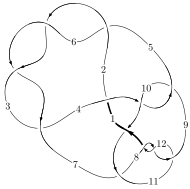
\includegraphics[width=112pt]{../../../GIT/diagram.site/Diagrams/png/1678_12a_0877.png}\\
\ \ \ A knot diagram\footnotemark}&
\allowdisplaybreaks
\textbf{Linearized knot diagam} \\
\cline{2-2}
 &
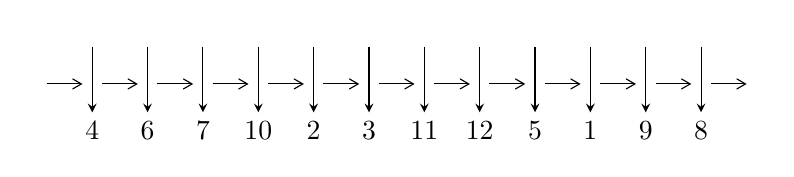
\begin{tikzpicture}[x=20pt, y=17pt]
	% nodes
	\node (C0) at (0, 0) {};
	\node (C1) at (1, 0) {};
	\node (C1U) at (1, +1) {};
	\node (C1D) at (1, -1) {4};

	\node (C2) at (2, 0) {};
	\node (C2U) at (2, +1) {};
	\node (C2D) at (2, -1) {6};

	\node (C3) at (3, 0) {};
	\node (C3U) at (3, +1) {};
	\node (C3D) at (3, -1) {7};

	\node (C4) at (4, 0) {};
	\node (C4U) at (4, +1) {};
	\node (C4D) at (4, -1) {10};

	\node (C5) at (5, 0) {};
	\node (C5U) at (5, +1) {};
	\node (C5D) at (5, -1) {2};

	\node (C6) at (6, 0) {};
	\node (C6U) at (6, +1) {};
	\node (C6D) at (6, -1) {3};

	\node (C7) at (7, 0) {};
	\node (C7U) at (7, +1) {};
	\node (C7D) at (7, -1) {11};

	\node (C8) at (8, 0) {};
	\node (C8U) at (8, +1) {};
	\node (C8D) at (8, -1) {12};

	\node (C9) at (9, 0) {};
	\node (C9U) at (9, +1) {};
	\node (C9D) at (9, -1) {5};

	\node (C10) at (10, 0) {};
	\node (C10U) at (10, +1) {};
	\node (C10D) at (10, -1) {1};

	\node (C11) at (11, 0) {};
	\node (C11U) at (11, +1) {};
	\node (C11D) at (11, -1) {9};

	\node (C12) at (12, 0) {};
	\node (C12U) at (12, +1) {};
	\node (C12D) at (12, -1) {8};
	\node (C13) at (13, 0) {};

	% arrows
	\draw[->,>={angle 60}]
	(C0) edge (C1) (C1) edge (C2) (C2) edge (C3) (C3) edge (C4) (C4) edge (C5) (C5) edge (C6) (C6) edge (C7) (C7) edge (C8) (C8) edge (C9) (C9) edge (C10) (C10) edge (C11) (C11) edge (C12) (C12) edge (C13) ;	\draw[->,>=stealth]
	(C1U) edge (C1D) (C2U) edge (C2D) (C3U) edge (C3D) (C4U) edge (C4D) (C5U) edge (C5D) (C6U) edge (C6D) (C7U) edge (C7D) (C8U) edge (C8D) (C9U) edge (C9D) (C10U) edge (C10D) (C11U) edge (C11D) (C12U) edge (C12D) ;
	\end{tikzpicture} \\
\hhline{~~} \\& 
\textbf{Solving Sequence} \\ \cline{2-2} 
 &
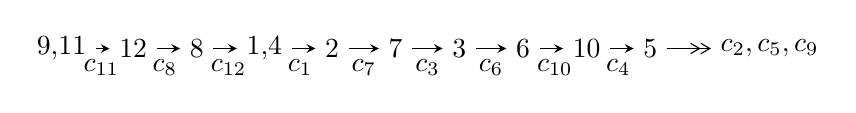
\begin{tikzpicture}[x=23pt, y=7pt]
	% node
	\node (A0) at (-1/8, 0) {9,11};
	\node (A1) at (1, 0) {12};
	\node (A2) at (2, 0) {8};
	\node (A3) at (49/16, 0) {1,4};
	\node (A4) at (33/8, 0) {2};
	\node (A5) at (41/8, 0) {7};
	\node (A6) at (49/8, 0) {3};
	\node (A7) at (57/8, 0) {6};
	\node (A8) at (65/8, 0) {10};
	\node (A9) at (73/8, 0) {5};
	\node (C1) at (1/2, -1) {$c_{11}$};
	\node (C2) at (3/2, -1) {$c_{8}$};
	\node (C3) at (5/2, -1) {$c_{12}$};
	\node (C4) at (29/8, -1) {$c_{1}$};
	\node (C5) at (37/8, -1) {$c_{7}$};
	\node (C6) at (45/8, -1) {$c_{3}$};
	\node (C7) at (53/8, -1) {$c_{6}$};
	\node (C8) at (61/8, -1) {$c_{10}$};
	\node (C9) at (69/8, -1) {$c_{4}$};
	\node (A10) at (11, 0) {$c_{2},c_{5},c_{9}$};

	% edge
	\draw[->,>=stealth]	
	(A0) edge (A1) (A1) edge (A2) (A2) edge (A3) (A3) edge (A4) (A4) edge (A5) (A5) edge (A6) (A6) edge (A7) (A7) edge (A8) (A8) edge (A9) ;
	\draw[->>,>={angle 60}]	
	(A9) edge (A10);
\end{tikzpicture} \\ 

\end{tabular} \\

\footnotetext{
The image of knot diagram is generated by the software ``\textbf{Draw programme}" developed by Andrew Bartholomew(\url{http://www.layer8.co.uk/maths/draw/index.htm\#Running-draw}), where we modified some parts for our purpose(\url{https://github.com/CATsTAILs/LinksPainter}).
}\phantom \\ \newline 
\centering \textbf{Ideals for irreducible components\footnotemark of $X_{\text{par}}$} 
 
\begin{align*}
I^u_{1}&=\langle 
- u^{68}+2 u^{67}+\cdots+2 b+1,\;u^{70}-3 u^{69}+\cdots+a-1,\;u^{71}-3 u^{70}+\cdots+u+1\rangle \\
I^u_{2}&=\langle 
u^2 b+b^2+b u+b+u,\;a,\;u^3+u^2+2 u+1\rangle \\
\\
\end{align*}
\raggedright * 2 irreducible components of $\dim_{\mathbb{C}}=0$, with total 77 representations.\\
\footnotetext{All coefficients of polynomials are rational numbers. But the coefficients are sometimes approximated in decimal forms when there is not enough margin.}
\newpage
\renewcommand{\arraystretch}{1}
\centering \section*{I. $I^u_{1}= \langle - u^{68}+2 u^{67}+\cdots+2 b+1,\;u^{70}-3 u^{69}+\cdots+a-1,\;u^{71}-3 u^{70}+\cdots+u+1 \rangle$}
\flushleft \textbf{(i) Arc colorings}\\
\begin{tabular}{m{7pt} m{180pt} m{7pt} m{180pt} }
\flushright $a_{9}=$&$\begin{pmatrix}0\\u\end{pmatrix}$ \\
\flushright $a_{11}=$&$\begin{pmatrix}1\\0\end{pmatrix}$ \\
\flushright $a_{12}=$&$\begin{pmatrix}1\\u^2\end{pmatrix}$ \\
\flushright $a_{8}=$&$\begin{pmatrix}u\\u^3+u\end{pmatrix}$ \\
\flushright $a_{1}=$&$\begin{pmatrix}u^2+1\\u^4+2 u^2\end{pmatrix}$ \\
\flushright $a_{4}=$&$\begin{pmatrix}- u^{70}+3 u^{69}+\cdots+9 u+1\\\frac{1}{2} u^{68}- u^{67}+\cdots+\frac{1}{2} u-\frac{1}{2}\end{pmatrix}$ \\
\flushright $a_{2}=$&$\begin{pmatrix}u^{17}+8 u^{15}+\cdots+u+2\\-\frac{1}{2} u^{68}+u^{67}+\cdots+\frac{1}{2} u+\frac{1}{2}\end{pmatrix}$ \\
\flushright $a_{7}=$&$\begin{pmatrix}u^3+2 u\\u^3+u\end{pmatrix}$ \\
\flushright $a_{3}=$&$\begin{pmatrix}-\frac{3}{2} u^{70}+\frac{9}{2} u^{69}+\cdots-20 u^2+\frac{7}{2} u\\2 u^{69}-5 u^{68}+\cdots-9 u^2- u\end{pmatrix}$ \\
\flushright $a_{6}=$&$\begin{pmatrix}\frac{1}{2} u^{70}-\frac{3}{2} u^{69}+\cdots-\frac{1}{2} u-2\\u^{68}-2 u^{67}+\cdots- u-1\end{pmatrix}$ \\
\flushright $a_{10}=$&$\begin{pmatrix}- u^6-3 u^4-2 u^2+1\\- u^8-4 u^6-4 u^4\end{pmatrix}$ \\
\flushright $a_{5}=$&$\begin{pmatrix}- u^{70}+3 u^{69}+\cdots+u-1\\2 u^{69}-\frac{11}{2} u^{68}+\cdots-\frac{5}{2} u-\frac{1}{2}\end{pmatrix}$\\&\end{tabular}
\flushleft \textbf{(ii) Obstruction class $= -1$}\\~\\
\flushleft \textbf{(iii) Cusp Shapes $= 4 u^{70}-\frac{23}{2} u^{69}+\cdots-3 u-\frac{39}{2}$}\\~\\
\newpage\renewcommand{\arraystretch}{1}
\flushleft \textbf{(iv) u-Polynomials at the component}\newline \\
\begin{tabular}{m{50pt}|m{274pt}}
Crossings & \hspace{64pt}u-Polynomials at each crossing \\
\hline $$\begin{aligned}c_{1}\end{aligned}$$&$\begin{aligned}
&u^{71}-18 u^{70}+\cdots+1020 u+207
\end{aligned}$\\
\hline $$\begin{aligned}c_{2},c_{3},c_{5}\\c_{6}\end{aligned}$$&$\begin{aligned}
&u^{71}+4 u^{70}+\cdots+2 u+1
\end{aligned}$\\
\hline $$\begin{aligned}c_{4},c_{9}\end{aligned}$$&$\begin{aligned}
&u^{71}- u^{70}+\cdots+96 u+64
\end{aligned}$\\
\hline $$\begin{aligned}c_{7}\end{aligned}$$&$\begin{aligned}
&u^{71}+3 u^{70}+\cdots+81 u+41
\end{aligned}$\\
\hline $$\begin{aligned}c_{8},c_{11},c_{12}\end{aligned}$$&$\begin{aligned}
&u^{71}-3 u^{70}+\cdots+u+1
\end{aligned}$\\
\hline $$\begin{aligned}c_{10}\end{aligned}$$&$\begin{aligned}
&u^{71}-15 u^{70}+\cdots-3735 u+1779
\end{aligned}$\\
\hline
\end{tabular}\\~\\
\newpage\renewcommand{\arraystretch}{1}
\flushleft \textbf{(v) Riley Polynomials at the component}\newline \\
\begin{tabular}{m{50pt}|m{274pt}}
Crossings & \hspace{64pt}Riley Polynomials at each crossing \\
\hline $$\begin{aligned}c_{1}\end{aligned}$$&$\begin{aligned}
&y^{71}+2 y^{70}+\cdots+577962 y-42849
\end{aligned}$\\
\hline $$\begin{aligned}c_{2},c_{3},c_{5}\\c_{6}\end{aligned}$$&$\begin{aligned}
&y^{71}-82 y^{70}+\cdots+18 y-1
\end{aligned}$\\
\hline $$\begin{aligned}c_{4},c_{9}\end{aligned}$$&$\begin{aligned}
&y^{71}+35 y^{70}+\cdots-48128 y-4096
\end{aligned}$\\
\hline $$\begin{aligned}c_{7}\end{aligned}$$&$\begin{aligned}
&y^{71}+5 y^{70}+\cdots-2459 y-1681
\end{aligned}$\\
\hline $$\begin{aligned}c_{8},c_{11},c_{12}\end{aligned}$$&$\begin{aligned}
&y^{71}+65 y^{70}+\cdots+21 y-1
\end{aligned}$\\
\hline $$\begin{aligned}c_{10}\end{aligned}$$&$\begin{aligned}
&y^{71}+25 y^{70}+\cdots+74059077 y-3164841
\end{aligned}$\\
\hline
\end{tabular}\\~\\
\newpage\flushleft \textbf{(vi) Complex Volumes and Cusp Shapes}
$$\begin{array}{c|c|c}  
\text{Solutions to }I^u_{1}& \I (\text{vol} + \sqrt{-1}CS) & \text{Cusp shape}\\
 \hline 
\begin{aligned}
u &= -0.298230 + 1.093620 I \\
a &= \phantom{-}0.472081 - 1.045720 I \\
b &= -0.791807 + 0.676221 I\end{aligned}
 & -6.03948 + 6.58052 I & \phantom{-0.000000 } 0 \\ \hline\begin{aligned}
u &= -0.298230 - 1.093620 I \\
a &= \phantom{-}0.472081 + 1.045720 I \\
b &= -0.791807 - 0.676221 I\end{aligned}
 & -6.03948 - 6.58052 I & \phantom{-0.000000 } 0 \\ \hline\begin{aligned}
u &= \phantom{-}0.102051 + 1.130360 I \\
a &= \phantom{-}1.069210 + 0.380589 I \\
b &= -0.72342 - 1.50387 I\end{aligned}
 & -7.48210 - 1.83544 I & \phantom{-0.000000 } 0 \\ \hline\begin{aligned}
u &= \phantom{-}0.102051 - 1.130360 I \\
a &= \phantom{-}1.069210 - 0.380589 I \\
b &= -0.72342 + 1.50387 I\end{aligned}
 & -7.48210 + 1.83544 I & \phantom{-0.000000 } 0 \\ \hline\begin{aligned}
u &= \phantom{-}0.001916 + 1.166800 I \\
a &= -0.976565 - 0.112077 I \\
b &= \phantom{-}0.156188 + 1.052190 I\end{aligned}
 & \phantom{-}0.637366 - 0.498211 I & \phantom{-0.000000 } 0 \\ \hline\begin{aligned}
u &= \phantom{-}0.001916 - 1.166800 I \\
a &= -0.976565 + 0.112077 I \\
b &= \phantom{-}0.156188 - 1.052190 I\end{aligned}
 & \phantom{-}0.637366 + 0.498211 I & \phantom{-0.000000 } 0 \\ \hline\begin{aligned}
u &= -0.245256 + 1.144100 I \\
a &= -0.485411 + 0.540876 I \\
b &= \phantom{-}0.176587 - 0.284101 I\end{aligned}
 & \phantom{-}1.43623 + 4.65090 I & \phantom{-0.000000 } 0 \\ \hline\begin{aligned}
u &= -0.245256 - 1.144100 I \\
a &= -0.485411 - 0.540876 I \\
b &= \phantom{-}0.176587 + 0.284101 I\end{aligned}
 & \phantom{-}1.43623 - 4.65090 I & \phantom{-0.000000 } 0 \\ \hline\begin{aligned}
u &= \phantom{-}0.435227 + 0.691944 I \\
a &= \phantom{-}2.00492 - 1.14289 I \\
b &= \phantom{-}1.037160 + 0.882341 I\end{aligned}
 & -5.01043 + 6.59194 I & -13.20650 - 2.66983 I \\ \hline\begin{aligned}
u &= \phantom{-}0.435227 - 0.691944 I \\
a &= \phantom{-}2.00492 + 1.14289 I \\
b &= \phantom{-}1.037160 - 0.882341 I\end{aligned}
 & -5.01043 - 6.59194 I & -13.20650 + 2.66983 I\\
 \hline 
 \end{array}$$\newpage$$\begin{array}{c|c|c}  
\text{Solutions to }I^u_{1}& \I (\text{vol} + \sqrt{-1}CS) & \text{Cusp shape}\\
 \hline 
\begin{aligned}
u &= \phantom{-}0.739876 + 0.307979 I \\
a &= -1.61074 + 2.29865 I \\
b &= -1.85820 + 1.64262 I\end{aligned}
 & -6.37543 - 10.74810 I & -15.6876 + 7.6872 I \\ \hline\begin{aligned}
u &= \phantom{-}0.739876 - 0.307979 I \\
a &= -1.61074 - 2.29865 I \\
b &= -1.85820 - 1.64262 I\end{aligned}
 & -6.37543 + 10.74810 I & -15.6876 - 7.6872 I \\ \hline\begin{aligned}
u &= \phantom{-}0.713231 + 0.321743 I \\
a &= \phantom{-}1.56422 - 1.71673 I \\
b &= \phantom{-}1.52378 - 0.87969 I\end{aligned}
 & \phantom{-}1.31275 - 8.10010 I & -12.6669 + 9.1497 I \\ \hline\begin{aligned}
u &= \phantom{-}0.713231 - 0.321743 I \\
a &= \phantom{-}1.56422 + 1.71673 I \\
b &= \phantom{-}1.52378 + 0.87969 I\end{aligned}
 & \phantom{-}1.31275 + 8.10010 I & -12.6669 - 9.1497 I \\ \hline\begin{aligned}
u &= -0.128401 + 1.230520 I \\
a &= \phantom{-}0.692003 + 0.027663 I \\
b &= \phantom{-}0.237864 - 0.428319 I\end{aligned}
 & \phantom{-}2.84553 + 1.96965 I & \phantom{-0.000000 } 0 \\ \hline\begin{aligned}
u &= -0.128401 - 1.230520 I \\
a &= \phantom{-}0.692003 - 0.027663 I \\
b &= \phantom{-}0.237864 + 0.428319 I\end{aligned}
 & \phantom{-}2.84553 - 1.96965 I & \phantom{-0.000000 } 0 \\ \hline\begin{aligned}
u &= -0.755331 + 0.102098 I \\
a &= \phantom{-}1.034040 - 0.668175 I \\
b &= \phantom{-}1.392900 - 0.229407 I\end{aligned}
 & -9.05815 - 2.69439 I & -17.2027 + 2.3657 I \\ \hline\begin{aligned}
u &= -0.755331 - 0.102098 I \\
a &= \phantom{-}1.034040 + 0.668175 I \\
b &= \phantom{-}1.392900 + 0.229407 I\end{aligned}
 & -9.05815 + 2.69439 I & -17.2027 - 2.3657 I \\ \hline\begin{aligned}
u &= \phantom{-}0.439054 + 0.620113 I \\
a &= -1.40227 + 1.08942 I \\
b &= -1.066550 - 0.215001 I\end{aligned}
 & \phantom{-}2.45899 + 4.08230 I & -9.92349 - 3.84314 I \\ \hline\begin{aligned}
u &= \phantom{-}0.439054 - 0.620113 I \\
a &= -1.40227 - 1.08942 I \\
b &= -1.066550 + 0.215001 I\end{aligned}
 & \phantom{-}2.45899 - 4.08230 I & -9.92349 + 3.84314 I\\
 \hline 
 \end{array}$$\newpage$$\begin{array}{c|c|c}  
\text{Solutions to }I^u_{1}& \I (\text{vol} + \sqrt{-1}CS) & \text{Cusp shape}\\
 \hline 
\begin{aligned}
u &= \phantom{-}0.674989 + 0.337780 I \\
a &= -1.34947 + 1.07393 I \\
b &= -0.989958 + 0.168014 I\end{aligned}
 & \phantom{-}2.62967 - 4.11560 I & -9.32664 + 4.02462 I \\ \hline\begin{aligned}
u &= \phantom{-}0.674989 - 0.337780 I \\
a &= -1.34947 - 1.07393 I \\
b &= -0.989958 - 0.168014 I\end{aligned}
 & \phantom{-}2.62967 + 4.11560 I & -9.32664 - 4.02462 I \\ \hline\begin{aligned}
u &= \phantom{-}0.581829 + 0.443643 I \\
a &= \phantom{-}0.680110 + 0.569291 I \\
b &= -0.245593 + 1.039410 I\end{aligned}
 & -1.63615 - 1.95033 I & -11.69879 + 3.63383 I \\ \hline\begin{aligned}
u &= \phantom{-}0.581829 - 0.443643 I \\
a &= \phantom{-}0.680110 - 0.569291 I \\
b &= -0.245593 - 1.039410 I\end{aligned}
 & -1.63615 + 1.95033 I & -11.69879 - 3.63383 I \\ \hline\begin{aligned}
u &= -0.665154 + 0.290764 I \\
a &= -0.66447 - 3.13003 I \\
b &= -1.39674 - 2.23065 I\end{aligned}
 & -8.61600 + 4.53223 I & -17.3927 - 4.7302 I \\ \hline\begin{aligned}
u &= -0.665154 - 0.290764 I \\
a &= -0.66447 + 3.13003 I \\
b &= -1.39674 + 2.23065 I\end{aligned}
 & -8.61600 - 4.53223 I & -17.3927 + 4.7302 I \\ \hline\begin{aligned}
u &= \phantom{-}0.468748 + 0.533484 I \\
a &= \phantom{-}0.676056 - 0.908880 I \\
b &= \phantom{-}0.924805 - 0.383040 I\end{aligned}
 & \phantom{-}3.46160 + 0.26111 I & -7.03816 + 2.83567 I \\ \hline\begin{aligned}
u &= \phantom{-}0.468748 - 0.533484 I \\
a &= \phantom{-}0.676056 + 0.908880 I \\
b &= \phantom{-}0.924805 + 0.383040 I\end{aligned}
 & \phantom{-}3.46160 - 0.26111 I & -7.03816 - 2.83567 I \\ \hline\begin{aligned}
u &= -0.700876 + 0.066926 I \\
a &= -0.320841 + 0.679183 I \\
b &= -0.468291 + 0.181364 I\end{aligned}
 & -1.81580 - 1.13539 I & -14.1583 + 5.8319 I \\ \hline\begin{aligned}
u &= -0.700876 - 0.066926 I \\
a &= -0.320841 - 0.679183 I \\
b &= -0.468291 - 0.181364 I\end{aligned}
 & -1.81580 + 1.13539 I & -14.1583 - 5.8319 I\\
 \hline 
 \end{array}$$\newpage$$\begin{array}{c|c|c}  
\text{Solutions to }I^u_{1}& \I (\text{vol} + \sqrt{-1}CS) & \text{Cusp shape}\\
 \hline 
\begin{aligned}
u &= -0.258326 + 1.292250 I \\
a &= \phantom{-}0.318100 - 0.050819 I \\
b &= \phantom{-}0.556440 - 0.515684 I\end{aligned}
 & \phantom{-}2.39024 + 2.32819 I & \phantom{-0.000000 } 0 \\ \hline\begin{aligned}
u &= -0.258326 - 1.292250 I \\
a &= \phantom{-}0.318100 + 0.050819 I \\
b &= \phantom{-}0.556440 + 0.515684 I\end{aligned}
 & \phantom{-}2.39024 - 2.32819 I & \phantom{-0.000000 } 0 \\ \hline\begin{aligned}
u &= -0.601819 + 0.265142 I \\
a &= \phantom{-}1.04132 + 2.29902 I \\
b &= \phantom{-}1.19691 + 1.23124 I\end{aligned}
 & -1.30198 + 2.69072 I & -15.0112 - 7.4612 I \\ \hline\begin{aligned}
u &= -0.601819 - 0.265142 I \\
a &= \phantom{-}1.04132 - 2.29902 I \\
b &= \phantom{-}1.19691 - 1.23124 I\end{aligned}
 & -1.30198 - 2.69072 I & -15.0112 + 7.4612 I \\ \hline\begin{aligned}
u &= -0.310470 + 1.307140 I \\
a &= -0.415211 - 0.292408 I \\
b &= -1.55166 + 1.02452 I\end{aligned}
 & -4.65881 + 1.15217 I & \phantom{-0.000000 } 0 \\ \hline\begin{aligned}
u &= -0.310470 - 1.307140 I \\
a &= -0.415211 + 0.292408 I \\
b &= -1.55166 - 1.02452 I\end{aligned}
 & -4.65881 - 1.15217 I & \phantom{-0.000000 } 0 \\ \hline\begin{aligned}
u &= \phantom{-}0.570835 + 0.293611 I \\
a &= \phantom{-}0.264731 - 0.690812 I \\
b &= -0.267146 + 0.080518 I\end{aligned}
 & -1.35568 - 1.48226 I & -14.0552 + 4.1663 I \\ \hline\begin{aligned}
u &= \phantom{-}0.570835 - 0.293611 I \\
a &= \phantom{-}0.264731 + 0.690812 I \\
b &= -0.267146 - 0.080518 I\end{aligned}
 & -1.35568 + 1.48226 I & -14.0552 - 4.1663 I \\ \hline\begin{aligned}
u &= \phantom{-}0.588263 + 0.180533 I \\
a &= \phantom{-}0.224002 + 1.011270 I \\
b &= \phantom{-}1.142880 + 0.126677 I\end{aligned}
 & -10.13840 - 0.81774 I & -16.4578 + 7.6947 I \\ \hline\begin{aligned}
u &= \phantom{-}0.588263 - 0.180533 I \\
a &= \phantom{-}0.224002 - 1.011270 I \\
b &= \phantom{-}1.142880 - 0.126677 I\end{aligned}
 & -10.13840 + 0.81774 I & -16.4578 - 7.6947 I\\
 \hline 
 \end{array}$$\newpage$$\begin{array}{c|c|c}  
\text{Solutions to }I^u_{1}& \I (\text{vol} + \sqrt{-1}CS) & \text{Cusp shape}\\
 \hline 
\begin{aligned}
u &= -0.344431 + 0.497662 I \\
a &= \phantom{-}2.83955 + 0.77238 I \\
b &= \phantom{-}0.94400 - 1.15638 I\end{aligned}
 & -7.51125 - 1.04755 I & -14.9755 - 1.6313 I \\ \hline\begin{aligned}
u &= -0.344431 - 0.497662 I \\
a &= \phantom{-}2.83955 - 0.77238 I \\
b &= \phantom{-}0.94400 + 1.15638 I\end{aligned}
 & -7.51125 + 1.04755 I & -14.9755 + 1.6313 I \\ \hline\begin{aligned}
u &= \phantom{-}0.226184 + 1.379720 I \\
a &= -0.265552 - 0.233022 I \\
b &= -1.54638 - 1.23737 I\end{aligned}
 & -5.13918 - 3.78426 I & \phantom{-0.000000 } 0 \\ \hline\begin{aligned}
u &= \phantom{-}0.226184 - 1.379720 I \\
a &= -0.265552 + 0.233022 I \\
b &= -1.54638 + 1.23737 I\end{aligned}
 & -5.13918 + 3.78426 I & \phantom{-0.000000 } 0 \\ \hline\begin{aligned}
u &= -0.197528 + 1.395160 I \\
a &= \phantom{-}0.029403 + 1.285120 I \\
b &= \phantom{-}1.66328 + 0.44069 I\end{aligned}
 & \phantom{-}4.62936 + 2.48780 I & \phantom{-0.000000 } 0 \\ \hline\begin{aligned}
u &= -0.197528 - 1.395160 I \\
a &= \phantom{-}0.029403 - 1.285120 I \\
b &= \phantom{-}1.66328 - 0.44069 I\end{aligned}
 & \phantom{-}4.62936 - 2.48780 I & \phantom{-0.000000 } 0 \\ \hline\begin{aligned}
u &= -0.23579 + 1.40424 I \\
a &= \phantom{-}0.70004 - 1.35070 I \\
b &= -1.87408 - 1.49381 I\end{aligned}
 & \phantom{-}4.03931 + 5.77114 I & \phantom{-0.000000 } 0 \\ \hline\begin{aligned}
u &= -0.23579 - 1.40424 I \\
a &= \phantom{-}0.70004 + 1.35070 I \\
b &= -1.87408 + 1.49381 I\end{aligned}
 & \phantom{-}4.03931 - 5.77114 I & \phantom{-0.000000 } 0 \\ \hline\begin{aligned}
u &= -0.14993 + 1.41755 I \\
a &= -0.89559 - 1.43480 I \\
b &= -1.71955 + 0.56930 I\end{aligned}
 & -1.60972 + 0.83337 I & \phantom{-0.000000 } 0 \\ \hline\begin{aligned}
u &= -0.14993 - 1.41755 I \\
a &= -0.89559 + 1.43480 I \\
b &= -1.71955 - 0.56930 I\end{aligned}
 & -1.60972 - 0.83337 I & \phantom{-0.000000 } 0\\
 \hline 
 \end{array}$$\newpage$$\begin{array}{c|c|c}  
\text{Solutions to }I^u_{1}& \I (\text{vol} + \sqrt{-1}CS) & \text{Cusp shape}\\
 \hline 
\begin{aligned}
u &= \phantom{-}0.22925 + 1.41881 I \\
a &= -0.097979 + 0.504327 I \\
b &= \phantom{-}0.265160 + 0.348113 I\end{aligned}
 & \phantom{-}4.15030 - 4.46057 I & \phantom{-0.000000 } 0 \\ \hline\begin{aligned}
u &= \phantom{-}0.22925 - 1.41881 I \\
a &= -0.097979 - 0.504327 I \\
b &= \phantom{-}0.265160 - 0.348113 I\end{aligned}
 & \phantom{-}4.15030 + 4.46057 I & \phantom{-0.000000 } 0 \\ \hline\begin{aligned}
u &= -0.25948 + 1.41528 I \\
a &= -1.29651 + 1.38162 I \\
b &= \phantom{-}2.11173 + 2.46119 I\end{aligned}
 & -3.16239 + 7.90974 I & \phantom{-0.000000 } 0 \\ \hline\begin{aligned}
u &= -0.25948 - 1.41528 I \\
a &= -1.29651 - 1.38162 I \\
b &= \phantom{-}2.11173 - 2.46119 I\end{aligned}
 & -3.16239 - 7.90974 I & \phantom{-0.000000 } 0 \\ \hline\begin{aligned}
u &= \phantom{-}0.25971 + 1.43435 I \\
a &= \phantom{-}0.054326 - 1.159680 I \\
b &= \phantom{-}1.282050 - 0.501952 I\end{aligned}
 & \phantom{-}8.30772 - 7.52976 I & \phantom{-0.000000 } 0 \\ \hline\begin{aligned}
u &= \phantom{-}0.25971 - 1.43435 I \\
a &= \phantom{-}0.054326 + 1.159680 I \\
b &= \phantom{-}1.282050 + 0.501952 I\end{aligned}
 & \phantom{-}8.30772 + 7.52976 I & \phantom{-0.000000 } 0 \\ \hline\begin{aligned}
u &= \phantom{-}0.28992 + 1.42978 I \\
a &= -0.58859 - 1.61725 I \\
b &= \phantom{-}2.63944 - 1.76837 I\end{aligned}
 & -0.8177 - 14.4909 I & \phantom{-0.000000 } 0 \\ \hline\begin{aligned}
u &= \phantom{-}0.28992 - 1.42978 I \\
a &= -0.58859 + 1.61725 I \\
b &= \phantom{-}2.63944 + 1.76837 I\end{aligned}
 & -0.8177 + 14.4909 I & \phantom{-0.000000 } 0 \\ \hline\begin{aligned}
u &= \phantom{-}0.27661 + 1.43275 I \\
a &= \phantom{-}0.25480 + 1.44753 I \\
b &= -2.05975 + 1.10091 I\end{aligned}
 & \phantom{-}6.93099 - 11.70450 I & \phantom{-0.000000 } 0 \\ \hline\begin{aligned}
u &= \phantom{-}0.27661 - 1.43275 I \\
a &= \phantom{-}0.25480 - 1.44753 I \\
b &= -2.05975 - 1.10091 I\end{aligned}
 & \phantom{-}6.93099 + 11.70450 I & \phantom{-0.000000 } 0\\
 \hline 
 \end{array}$$\newpage$$\begin{array}{c|c|c}  
\text{Solutions to }I^u_{1}& \I (\text{vol} + \sqrt{-1}CS) & \text{Cusp shape}\\
 \hline 
\begin{aligned}
u &= \phantom{-}0.15789 + 1.45296 I \\
a &= \phantom{-}0.407502 + 0.650068 I \\
b &= -1.38045 + 0.86766 I\end{aligned}
 & \phantom{-}9.77362 - 1.97022 I & \phantom{-0.000000 } 0 \\ \hline\begin{aligned}
u &= \phantom{-}0.15789 - 1.45296 I \\
a &= \phantom{-}0.407502 - 0.650068 I \\
b &= -1.38045 - 0.86766 I\end{aligned}
 & \phantom{-}9.77362 + 1.97022 I & \phantom{-0.000000 } 0 \\ \hline\begin{aligned}
u &= \phantom{-}0.13021 + 1.45714 I \\
a &= -0.082139 - 1.018390 I \\
b &= \phantom{-}1.51015 - 0.72465 I\end{aligned}
 & \phantom{-}9.02491 + 2.18165 I & \phantom{-0.000000 } 0 \\ \hline\begin{aligned}
u &= \phantom{-}0.13021 - 1.45714 I \\
a &= -0.082139 + 1.018390 I \\
b &= \phantom{-}1.51015 + 0.72465 I\end{aligned}
 & \phantom{-}9.02491 - 2.18165 I & \phantom{-0.000000 } 0 \\ \hline\begin{aligned}
u &= \phantom{-}0.19927 + 1.44971 I \\
a &= -0.666580 + 0.052748 I \\
b &= \phantom{-}0.707982 - 0.886535 I\end{aligned}
 & \phantom{-}4.44129 - 4.75957 I & \phantom{-0.000000 } 0 \\ \hline\begin{aligned}
u &= \phantom{-}0.19927 - 1.44971 I \\
a &= -0.666580 - 0.052748 I \\
b &= \phantom{-}0.707982 + 0.886535 I\end{aligned}
 & \phantom{-}4.44129 + 4.75957 I & \phantom{-0.000000 } 0 \\ \hline\begin{aligned}
u &= \phantom{-}0.10296 + 1.46363 I \\
a &= -0.336387 + 1.303930 I \\
b &= -1.45662 + 0.53173 I\end{aligned}
 & \phantom{-}1.83471 + 4.95872 I & \phantom{-0.000000 } 0 \\ \hline\begin{aligned}
u &= \phantom{-}0.10296 - 1.46363 I \\
a &= -0.336387 - 1.303930 I \\
b &= -1.45662 - 0.53173 I\end{aligned}
 & \phantom{-}1.83471 - 4.95872 I & \phantom{-0.000000 } 0 \\ \hline\begin{aligned}
u &= -0.401557 + 0.210000 I \\
a &= -1.79421 - 0.99079 I \\
b &= -0.818427 - 0.029641 I\end{aligned}
 & -0.590115 + 0.032455 I & -12.52222 + 0.27337 I \\ \hline\begin{aligned}
u &= -0.401557 - 0.210000 I \\
a &= -1.79421 + 0.99079 I \\
b &= -0.818427 + 0.029641 I\end{aligned}
 & -0.590115 - 0.032455 I & -12.52222 - 0.27337 I\\
 \hline 
 \end{array}$$\newpage$$\begin{array}{c|c|c}  
\text{Solutions to }I^u_{1}& \I (\text{vol} + \sqrt{-1}CS) & \text{Cusp shape}\\
 \hline 
\begin{aligned}
u &= -0.270889\phantom{ +0.000000I} \\
a &= -2.15579\phantom{ +0.000000I} \\
b &= -0.509358\phantom{ +0.000000I}\end{aligned}
 & -0.645856\phantom{ +0.000000I} & -14.8110\phantom{ +0.000000I}\\
 \hline 
 \end{array}$$\newpage\newpage\renewcommand{\arraystretch}{1}
\centering \section*{II. $I^u_{2}= \langle u^2 b+b^2+b u+b+u,\;a,\;u^3+u^2+2 u+1 \rangle$}
\flushleft \textbf{(i) Arc colorings}\\
\begin{tabular}{m{7pt} m{180pt} m{7pt} m{180pt} }
\flushright $a_{9}=$&$\begin{pmatrix}0\\u\end{pmatrix}$ \\
\flushright $a_{11}=$&$\begin{pmatrix}1\\0\end{pmatrix}$ \\
\flushright $a_{12}=$&$\begin{pmatrix}1\\u^2\end{pmatrix}$ \\
\flushright $a_{8}=$&$\begin{pmatrix}u\\- u^2- u-1\end{pmatrix}$ \\
\flushright $a_{1}=$&$\begin{pmatrix}u^2+1\\u^2+u+1\end{pmatrix}$ \\
\flushright $a_{4}=$&$\begin{pmatrix}0\\b\end{pmatrix}$ \\
\flushright $a_{2}=$&$\begin{pmatrix}u^2+1\\2 u^2- b+2 u+2\end{pmatrix}$ \\
\flushright $a_{7}=$&$\begin{pmatrix}- u^2-1\\- u^2- u-1\end{pmatrix}$ \\
\flushright $a_{3}=$&$\begin{pmatrix}u^2 b+b u+2 b\\2 b\end{pmatrix}$ \\
\flushright $a_{6}=$&$\begin{pmatrix}- u^2 b- b u-2 b\\u^2-2 b+u+1\end{pmatrix}$ \\
\flushright $a_{10}=$&$\begin{pmatrix}0\\u\end{pmatrix}$ \\
\flushright $a_{5}=$&$\begin{pmatrix}0\\b\end{pmatrix}$\\&\end{tabular}
\flushleft \textbf{(ii) Obstruction class $= 1$}\\~\\
\flushleft \textbf{(iii) Cusp Shapes $= b u-3 u^2- b-5 u-20$}\\~\\
\newpage\renewcommand{\arraystretch}{1}
\flushleft \textbf{(iv) u-Polynomials at the component}\newline \\
\begin{tabular}{m{50pt}|m{274pt}}
Crossings & \hspace{64pt}u-Polynomials at each crossing \\
\hline $$\begin{aligned}c_{1},c_{2},c_{3}\end{aligned}$$&$\begin{aligned}
&(u^2+u-1)^3
\end{aligned}$\\
\hline $$\begin{aligned}c_{4},c_{9}\end{aligned}$$&$\begin{aligned}
&u^6
\end{aligned}$\\
\hline $$\begin{aligned}c_{5},c_{6}\end{aligned}$$&$\begin{aligned}
&(u^2- u-1)^3
\end{aligned}$\\
\hline $$\begin{aligned}c_{7},c_{10}\end{aligned}$$&$\begin{aligned}
&(u^3+u^2-1)^2
\end{aligned}$\\
\hline $$\begin{aligned}c_{8}\end{aligned}$$&$\begin{aligned}
&(u^3- u^2+2 u-1)^2
\end{aligned}$\\
\hline $$\begin{aligned}c_{11},c_{12}\end{aligned}$$&$\begin{aligned}
&(u^3+u^2+2 u+1)^2
\end{aligned}$\\
\hline
\end{tabular}\\~\\
\newpage\renewcommand{\arraystretch}{1}
\flushleft \textbf{(v) Riley Polynomials at the component}\newline \\
\begin{tabular}{m{50pt}|m{274pt}}
Crossings & \hspace{64pt}Riley Polynomials at each crossing \\
\hline $$\begin{aligned}c_{1},c_{2},c_{3}\\c_{5},c_{6}\end{aligned}$$&$\begin{aligned}
&(y^2-3 y+1)^3
\end{aligned}$\\
\hline $$\begin{aligned}c_{4},c_{9}\end{aligned}$$&$\begin{aligned}
&y^6
\end{aligned}$\\
\hline $$\begin{aligned}c_{7},c_{10}\end{aligned}$$&$\begin{aligned}
&(y^3- y^2+2 y-1)^2
\end{aligned}$\\
\hline $$\begin{aligned}c_{8},c_{11},c_{12}\end{aligned}$$&$\begin{aligned}
&(y^3+3 y^2+2 y-1)^2
\end{aligned}$\\
\hline
\end{tabular}\\~\\
\newpage\flushleft \textbf{(vi) Complex Volumes and Cusp Shapes}
$$\begin{array}{c|c|c}  
\text{Solutions to }I^u_{2}& \I (\text{vol} + \sqrt{-1}CS) & \text{Cusp shape}\\
 \hline 
\begin{aligned}
u &= -0.215080 + 1.307140 I \\
a &= \phantom{-0.000000 } 0 \\
b &= -0.542287 + 0.460350 I\end{aligned}
 & \phantom{-}2.03717 + 2.82812 I & -13.8803 - 6.1171 I \\ \hline\begin{aligned}
u &= -0.215080 + 1.307140 I \\
a &= \phantom{-0.000000 } 0 \\
b &= \phantom{-}1.41973 - 1.20521 I\end{aligned}
 & -5.85852 + 2.82812 I & -14.0872 - 1.5287 I \\ \hline\begin{aligned}
u &= -0.215080 - 1.307140 I \\
a &= \phantom{-0.000000 } 0 \\
b &= -0.542287 - 0.460350 I\end{aligned}
 & \phantom{-}2.03717 - 2.82812 I & -13.8803 + 6.1171 I \\ \hline\begin{aligned}
u &= -0.215080 - 1.307140 I \\
a &= \phantom{-0.000000 } 0 \\
b &= \phantom{-}1.41973 + 1.20521 I\end{aligned}
 & -5.85852 - 2.82812 I & -14.0872 + 1.5287 I \\ \hline\begin{aligned}
u &= -0.569840\phantom{ +0.000000I} \\
a &= \phantom{-0.000000 } 0 \\
b &= -1.22142\phantom{ +0.000000I}\end{aligned}
 & -9.99610\phantom{ +0.000000I} & -16.2080\phantom{ +0.000000I} \\ \hline\begin{aligned}
u &= -0.569840\phantom{ +0.000000I} \\
a &= \phantom{-0.000000 } 0 \\
b &= \phantom{-}0.466540\phantom{ +0.000000I}\end{aligned}
 & -2.10041\phantom{ +0.000000I} & -18.8570\phantom{ +0.000000I}\\
 \hline 
 \end{array}$$\newpage
\newpage\renewcommand{\arraystretch}{1}
\centering \section*{ III. u-Polynomials}
\begin{tabular}{m{50pt}|m{274pt}}
Crossings & \hspace{64pt}u-Polynomials at each crossing \\
\hline $$\begin{aligned}c_{1}\end{aligned}$$&$\begin{aligned}
&((u^2+u-1)^3)(u^{71}-18 u^{70}+\cdots+1020 u+207)
\end{aligned}$\\
\hline $$\begin{aligned}c_{2},c_{3}\end{aligned}$$&$\begin{aligned}
&((u^2+u-1)^3)(u^{71}+4 u^{70}+\cdots+2 u+1)
\end{aligned}$\\
\hline $$\begin{aligned}c_{4},c_{9}\end{aligned}$$&$\begin{aligned}
&u^6(u^{71}- u^{70}+\cdots+96 u+64)
\end{aligned}$\\
\hline $$\begin{aligned}c_{5},c_{6}\end{aligned}$$&$\begin{aligned}
&((u^2- u-1)^3)(u^{71}+4 u^{70}+\cdots+2 u+1)
\end{aligned}$\\
\hline $$\begin{aligned}c_{7}\end{aligned}$$&$\begin{aligned}
&((u^3+u^2-1)^2)(u^{71}+3 u^{70}+\cdots+81 u+41)
\end{aligned}$\\
\hline $$\begin{aligned}c_{8}\end{aligned}$$&$\begin{aligned}
&((u^3- u^2+2 u-1)^2)(u^{71}-3 u^{70}+\cdots+u+1)
\end{aligned}$\\
\hline $$\begin{aligned}c_{10}\end{aligned}$$&$\begin{aligned}
&((u^3+u^2-1)^2)(u^{71}-15 u^{70}+\cdots-3735 u+1779)
\end{aligned}$\\
\hline $$\begin{aligned}c_{11},c_{12}\end{aligned}$$&$\begin{aligned}
&((u^3+u^2+2 u+1)^2)(u^{71}-3 u^{70}+\cdots+u+1)
\end{aligned}$\\
\hline
\end{tabular}\newpage\renewcommand{\arraystretch}{1}
\centering \section*{ IV. Riley Polynomials}
\begin{tabular}{m{50pt}|m{274pt}}
Crossings & \hspace{64pt}Riley Polynomials at each crossing \\
\hline $$\begin{aligned}c_{1}\end{aligned}$$&$\begin{aligned}
&((y^2-3 y+1)^3)(y^{71}+2 y^{70}+\cdots+577962 y-42849)
\end{aligned}$\\
\hline $$\begin{aligned}c_{2},c_{3},c_{5}\\c_{6}\end{aligned}$$&$\begin{aligned}
&((y^2-3 y+1)^3)(y^{71}-82 y^{70}+\cdots+18 y-1)
\end{aligned}$\\
\hline $$\begin{aligned}c_{4},c_{9}\end{aligned}$$&$\begin{aligned}
&y^6(y^{71}+35 y^{70}+\cdots-48128 y-4096)
\end{aligned}$\\
\hline $$\begin{aligned}c_{7}\end{aligned}$$&$\begin{aligned}
&((y^3- y^2+2 y-1)^2)(y^{71}+5 y^{70}+\cdots-2459 y-1681)
\end{aligned}$\\
\hline $$\begin{aligned}c_{8},c_{11},c_{12}\end{aligned}$$&$\begin{aligned}
&((y^3+3 y^2+2 y-1)^2)(y^{71}+65 y^{70}+\cdots+21 y-1)
\end{aligned}$\\
\hline $$\begin{aligned}c_{10}\end{aligned}$$&$\begin{aligned}
&((y^3- y^2+2 y-1)^2)(y^{71}+25 y^{70}+\cdots+7.40591\times10^{7} y-3164841)
\end{aligned}$\\
\hline
\end{tabular}
\vskip 2pc
\end{document}